\documentclass{standalone}
\usepackage{tikz}
\usetikzlibrary{positioning, calc, intersections}

\tikzstyle{vnode}=[circle, draw, very thick, minimum size=5pt]
\tikzstyle{check}=[rectangle,minimum size=6mm,rounded corners=1mm,
                          % The rest
                          very thick,draw=black]
\begin{document}
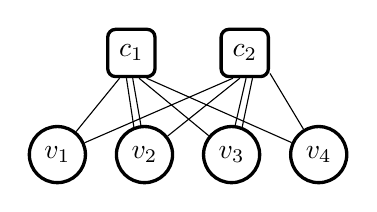
\begin{tikzpicture}[auto]
  % Define styles for variable and check nodes
  
  % Place variable nodes on the bottom row
  \node[vnode] (v1) at (0,0) {$v_1$};
  \node[vnode, right = 10pt of v1.east] (v2) {$v_2$};
  \node[vnode, right = 10pt of v2.east] (v3) {$v_3$};
  \node[vnode, right = 10pt of v3.east] (v4) {$v_4$};
  
  % Place check nodes with particularly close spacing
  \node[check, above right = 20pt and 10pt of v1.north east] (c1) {$c_1$};
  \node[check, above left = 20pt and 10pt of v4.north west] (c2) {$c_2$};

  \path [rounded corners=.96cm, name path=A] (c1.south)|-(c1.east);
  \path [name path=B] (c1.east -| c1.south) -- (c1.south -| c1.east);
  \coordinate[name intersections={of=A and B, by=c1SE}];
  



\path (v1) edge (c1.-115);
\path (v2.111) edge (c1.-101);
\path (v2.97) edge (c1.-87);
\path (v3) edge (c1.-73);
\path (v4) edge (c1.-59);

\path (v1) edge (c2.-115);
\path (v2) edge (c2.-101);
\path (v3.83) edge (c2.-87);
\path (v3.69) edge (c2.-73);
\path (v4) edge (c2.-759);
  % \path (v1.65) edge (c1.south west);
  % \path (v1.45) edge (c1.-125);
  % \path (v1) edge (c1);
  % \path (v1) edge (c1);
  
\end{tikzpicture}
\end{document}